% a mashup of hipstercv, friggeri and twenty cv
% https://www.latextemplates.com/template/twenty-seconds-resumecv
% https://www.latextemplates.com/template/friggeri-resume-cv

\documentclass[allblack]{simplehipstercv}
% available options are: darkhipster, lighthipster, pastel, allblack, grey, verylight, withoutsidebar
% withoutsidebar
%\usepackage[utf8]{inputenc}
\usepackage[default]{raleway}
\usepackage[includefoot,margin = 0.5cm, a4paper]{geometry}%margin=1cm
\usepackage{hyperref}
\usepackage{fancyhdr}
\usepackage{blindtext}
\usepackage{lastpage}
\usepackage{paracol}
%------------------------------------------------------------------ Variablen

\newlength{\rightcolwidth}
\newlength{\leftcolwidth}
\setlength{\leftcolwidth}{0.75\textwidth}
\setlength{\rightcolwidth}{0.75\textwidth}

%------------------------------------------------------------------
\title{Private Sector CV}
\author{Jared Holland}
\date{May 2024}


\begin{document}

%-------------------------------------------------------------

\section*{}

\simpleheader{headercolour}{Jared}{Holland}{Franklin, North Carolina 28734}{white}

\pagestyle{fancy}
\fancyhf{}
\rfoot{\thepage \hspace{12pt}}
%-------------------------------------------------------------

% this has to be here so the paracols starts..
\subsection*{}
\vspace{5em}

\setlength{\columnsep}{2cm}
\columnratio{0.25}[0.75]
\begin{paracol}{2}
\hbadness5000

%\backgroundcolor{c[1]}[rgb]{1,1,0.8} % cream yellow for column-1 %\backgroundcolor{g}[rgb]{0.8,1,1} % \backgroundcolor{l}[rgb]{0,0,0.7} % dark blue for left margin

\paracolbackgroundoptions
% 0.9,0.9,0.9 -- 0.8,0.8,0.8


\footnotesize
{\setasidefontcolour
\flushleft
\bg{cvgreen}{white}{About me}\\[0.5em]
    {\footnotesize
    A results-driven engineering
    professional with a strong
    foundation in Mechanical Engineering
    and a keen interest in the
    advancement of aerospace technology,
    seeking to leverage my years of
    hands-on industry experience and
    education to contribute to the NASA Langley Research Center.}\\
\bigskip
\bg{cvgreen}{white}{Areas of specialization} \\[0.5em]

    3D CAD Software ~•~ CFD Simulation ~•~ FEA Analysis ~•~ Python ~•~ MATLAB/Octave ~•~ 3D Printing Technology ~•~ Mechanical Drawings ~•~ CNC Machining\\

\bigskip
\bg{cvgreen}{white}{Soft Skills} \\[0.5em]

    Teamwork Oriented ~•~ Strong Communicator ~•~ Leadership ~•~ Organized \\

\bigskip

\bg{cvgreen}{white}{Interests}\\[0.5em]

Blacksmithing, 3D printing, Robotics, CNC Machining,
Hiking, Plants, Guitar\\
\bigskip

\infobubble{\faEnvelope}{cvgreen}{white}{jsholland231@gmail.com}
\infobubble{\faPhone}{cvgreen}{white}{828-342-7788}

%\phantom{turn the page}
%\phantom{turn the page}
}
%----------------------------------------------------------- Switch to second column
\switchcolumn
\section*{GS:11 Qualifications}
    This is my application for the Equipment Facilities and Services Specialist at NASA Langley Research
    Center (Job Code: 805472500). I have 5 years of experience in various engineering industries. I have
    delivered on several projects, carefully analyzing safety, cost, and manufacturability. I have 8 years
    of experience in fabrication using multiple materials. Electrical design is where I got my start and my skills
    have grown with me into the present day.\\
    \\
    During my employment at TekTone: Sound \& Signal I provided technical support and documentation
    to more than 10 projects during my 4 years of continuous employment. Many of the test fixtures and apparatus that I designed required the usage of production drawings, specifications provided by myself or
    the engineering team, and test reports usually written in Microsoft Word or LATEX. One root cause analysis project, in particular, where I used my report writing skills extensively, helped to save TekTone several
    1000s of dollars in producing corrective parts for one of their high-volume products. I provided equipment
    maintenance on all of the testers I designed at TekTone, but while I was in the manufacturing department
    I was trained in the operation and maintenance of all key equipment in the automation line.\\
    \\
    During my undergraduate education, I further refined and used my engineering skills to great effect. This
    often was commended on all accounts. My achievements in class led me to be handpicked for the Cube-
    Sat capstone project offered during my senior year. I led the mechanical design and fabrication efforts on
    that team, resulting in meeting the goals of our sponsor Destination SPACE Inc. This experience added to
    my knowledge of aerospace engineering.\\
    \\
    My skills and experience have been proven in my career. Based on my experiences I am qualified to
    perform the duties listed in the job description. % Treat the end like a the conclusion of a thesis 

\section*{Volunteer Work}
\begin{tabular}{r| p{0.5\textwidth} c}
    \cvevent{June 2023}{Western Carolina University: Weather Balloon Launch}{}{Cullowhee, NC \color{cvred}}{
        \begin{itemize}
            \item Assisted in the setup of a weather balloon equipped with temperature sensors, Geiger counter, and camera.
            \item Was a part of the recovery team that chased the balloon from Western's campus to Greer, South Carolina.
        \end{itemize}
    
    }
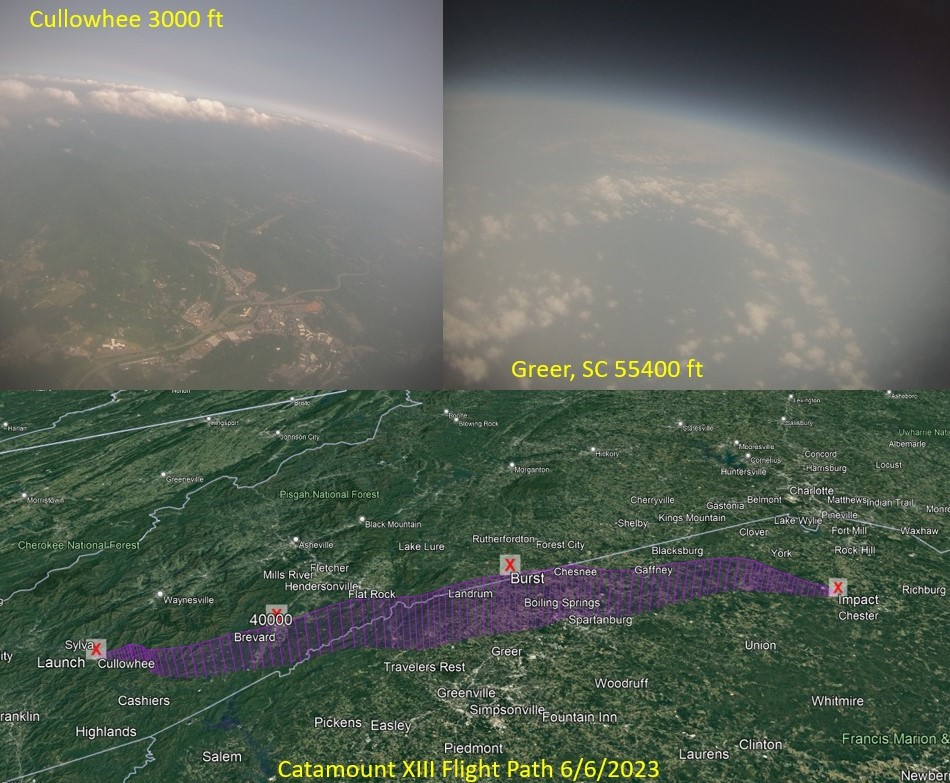
\includegraphics[width=0.5\textwidth]{06062023_Collage.jpg}\\  
\end{tabular}
%%%%%%%%%%%%%%%%%%%%%%%%%%%%%%%%%%%%%%%%%%%%%%%%%%%%%%%%%%%%%% Employment History
\section*{Employment History}
\begin{tabular}{r| p{0.5\textwidth} c} %%% LEIDOS
    \cvevent{2023--2024}{Leidos: Power Distribution}{Power Distribution Engineer}{Asheville, NC \color{cvred}}{
        \begin{itemize}
            \item Developed power pole layouts in collaboration with Duke Energy, 
            demonstrating expertise in \textbf{engineering design principles} and \textbf{adherence to industry standards}.
            \item Managed bill of materials to ensure the \textbf{reliability} and \textbf{efficiency} of distribution circuits, 
            contributing to the seamless operation of the North Carolina power grid.
            \item Utilized \textbf{Maximo} to facilitate effective communication and coordination of permitting efforts and vital design information, 
            optimizing construction processes for field personnel and improving the long term \textbf{safety} to the environment.
            \item Performed field survey work to inspect and gather data on each power pole assigned to the Leidos Asheville 
            office so that the engineering team had sufficient data to start their designs.
            \item Leveraged \textbf{ArcGIS} to generate preliminary designs, proactively identifying and addressing potential environmental, structural, 
            and permitting challenges before initiating the formal design processes.
        \end{itemize}
    } \\
    %%%%%%%%%%%%%%%%%%%%%%%%%%%%%%%%%%%%%%%%%%%%%%%%%%%%%%%% Mech: TekTone
    \cvevent{2022--2023}{TekTone: Sound \& Signal}{Mechanical Engineering Intern}{Franklin, NC \color{cvred}}{
        \begin{itemize}
            \item Led the mechanical design for two anti-vandal nurse call stations, overseeing the entire life cycle from conceptualization to successful product launch. 
            \textbf{Gantt Project} was utilized heavily for efficient project management during this assignment. It was indispensable in properly allocating team resources and ensuring the timely achievement of project milestones.
            \item Produced quality \textbf{mechanical drawings} for the 2 antivandal nurse call stations and for the various test fixtures I designed   
            %%%%%%%%%%%%%%%%%%%%%%%%%%%%%%%%5
            \item Spearheaded the usage of 3D printing technology for use in the \textbf{fabrication} of high-quality \textbf{test fixtures} that enhanced production processes and turnaround times. During the design phase 
            collaboration with the production floor workers and machine shop personnel was instrumental in ensuring that \textbf{each test article} or \textbf{tool} was built to fit their design needs and to ensure manufacturability. 
            %%%%%%%%%%%%%%%%%%%%%%%%%%%%%%%%5
            \item Implemented 3D printing technology that aided in producing corrective parts for high-volume products resulting in savings; avoiding shipping issues and unnecessarily ordering injection molds. 
            \item Standardized the use of the \textbf{UL200B} \textbf{safety standards} for 3D printing.
            \item Created \textbf{test procedures} for more than 3 test fixtures I designed.  
            \item Conducted research projects using the \textbf{scientific method} that involved root cause analysis among other optimization studies. These projects used software tools such as \textbf{R Studio}, \textbf{Python},
            and \textbf{MATLAB/Octave} to produce high-quality graphs and figures that were then organized in \textbf{\LaTeX{}} for presentation to management and interested parties.
        \end{itemize}
    } \\ 
    %%%%%%%%%%%%%%%%%%%%%%%%%%%%%%%%%%%%%%%%%%%%%%%%%%%%%%%% Manufac: TekTone
    \cvevent{2019--2022}{TekTone: Sound \& Signal}{Manufacturing Engineering Intern}{Franklin, NC \color{cvred}}{
        \begin{itemize}
            \item Worked with other technicians to run various parts of the automation line to ensure we met the production quota. 
            This fostered a culture among the automated assembly line workers of \textbf{inclusiveness}, \textbf{excellence}, and \textbf{teamwork}. 
            We viewed our fellow workers’ success as our own success. Our technician lead never had to worry about our competence.
            \item Trained to \textbf{operate} and \textbf{maintain} the \textbf{Panasonic pick n place equipment}, \textbf{Automated Optical Inspection equipment}, and \textbf{SPEA 4080} high volume test machine. 
            \item Preformed a broad scope of duties. These duties included gathering design metrics, creating design concepts, producing mechanical \textbf{designs},
            electrical \textbf{designs}, fabrication (\textbf{buildup}), optimization, and \textbf{modification} of various \textbf{experimental} test fixures and tools.  
            \item Developed Python script modules for KiCAD circuit board design software, enabling seamless communication between engineering and production teams. 
            These modules generated usable files for the \textbf{Panasonic automation line} and the \textbf{SPEA 4080}, \textbf{improving design efficiency}, and \textbf{reducing errors in manufacturing}.
            \item Demonstrated initiative and dedication, progressing from an electronics assembly worker to a Manufacturing Engineering Intern within 2 months, 
            showcasing adaptability and a strong work ethic. 
        \end{itemize}
    }
\end{tabular}
\newpage
%\vspace{2em}
\section*{Education}
    %%%%%%%%%%%%%%%%%%%%%%%%%%%%%%%%%%%%%%%%%%%%%%%%%%%%%% WCU: BSE|Mech
    \begin{tabular}{r| p{0.5\textwidth} c}
        \cvevent{2019--2023}{Bachelors In Mechanical Engineering}{Western Carolina University}{Cullowhee, NC \color{cvred}}{
            \newline    
            \textbf{CubeSat Capstone Project}
            \newline
            \textit{fall and spring senior semesters}
            \begin{itemize}
                \item Hand-picked by the WCU rapid center staff for my demonstrated knowledge and competence in heat transfer analysis and structural design.
                \item Led a multidisciplinary team in developing the mechanical design for the CubeSat frame.
                \item Conducted extensive preliminary research in \textbf{CubeSat operational systems}. We took the necessary time to evaluate CubeSat flight system hardware 
                devices such as \textbf{boosters}, \textbf{reaction wheels}, \textbf{magnetorquers}, \textbf{Inertial Measurement Units}, and \textbf{Startracker} amongst some of the \textbf{spacecraft systems} we reviewed. 
                This contributed to successfully implementing hardware within our allocated time frame without wasting our budget or time.
                \item Utilized programming skills in VS Code to \textbf{support electrical engineering team members} with logic board programming and \textbf{conducted design audits of circuit boards} 
                assessing \textbf{system performance}, \textbf{layout}, \textbf{operational limits}, \textbf{reliability}, and \textbf{manufacturability} using KiCAD circuit board design software.
                \item Preformed the design and \textbf{fabrication} of the mechanical frame in the \textbf{Western Carolina University machine shop}, ensuring compliance with project requirements and specifications provided by \textbf{ISO17770}. 
                \item Assisted in maintianing project documentation that clearly outlined the lessons and sucesses found during the project. This
                allowed for better tracking of milestones and goal completion.
                \item Facilitated \textbf{communication} with sponsors and engineering mentors, providing regular updates on the firmware, mechanical design, and fabrication progress. 
                This communication was pivotal in guiding project direction so that our team met sponsor objectives.
            \end{itemize}
            \textbf{Academic Achievements}
            \begin{itemize}
                \item Dean's List recognition for outstanding academic performance.
                \item Graduated with a minor in math.
            \end{itemize}
            \textbf{Technical Skills Acquired}
            \begin{itemize}
                \item Proficiency in \textbf{Finite Element Analysis (FEA)} for gantries and steel structures in both \textbf{CREO parametric} and \textbf{Ansys}.
                \item Advanced proficiency in 3D modeling and assembly using Creo Parametric and Autodesk Inventor.
                \item Foundational understanding of \textbf{Computational Fluid Dynamics (CFD)} analysis using \textbf{Ansys software}.
                \item Hands-on experience in \textbf{waterjet cutting} production processes, \textbf{inspection}, and maintenance.
                \item Conducted an \textbf{independent study with Tektone: Sound \& Signal} to determine the thermal loads on their nurse call system hardware. 
                This required extensive use of \textbf{MATLAB} and \textbf{FLIR} devices to determine if the electronics needed extra ventilation or cooling.
                \item Assisted in \textbf{repair}, \textbf{modification}, and \textbf{maintenance} of 3D printers within the 3D print lab.
                \item Utilized CNC Machining for milling \textbf{wood} and \textbf{plastic} parts.
                \item Learned Aluminum \textbf{TIG welding} for the CubeSat project. 
            \end{itemize}
        } \\
        %%%%%%%%%%%%%%%%%%%%%%%%%%%%%%%%%%%%%% SCC: AS
        \cvevent{2015--2019}{Associates in Science}{Southwestern Community College}{Sylva, NC \color{cvred}}{
            \begin{itemize}
                \item Developed proficiency in \textbf{3D printer design and modification}, culminating in the construction of a customized 3D printer from scratch.
                \item Applied knowledge in hobby electronics and utilized \textbf{KiCAD} for electronics design projects.
                \item Acquired practical skills in \textbf{metalworking} and \textbf{blacksmithing}, including basic practices for \textbf{MIG} and \textbf{ARC} welding techniques.
                \item Gained proficiency in programming languages including \textbf{C++}, \textbf{C\#}, \textbf{Python}, \textbf{Arduino}, and \textbf{G-code}, enabling customization of custom 3D printer firmware.
                \item Developed strong foundations in 3D CAD software such as \textbf{FreeCAD}, \textbf{Autodesk Inventor}, and \textbf{Blender}, utilizing these skills to design and produce 3D printable products that funded workshop upgrades and materials.
            \end{itemize}
        }
\end{tabular}
\vspace{1em}
%%%%%%%%%%%%%%%%%%%%%%%%%%%%%%%%%%%%%%%%%%%%%%%%%%%%%%%%%%%%%%%%%%%%%%%%%%%%
\section*{Software Experience and Technical Skills}
    \begin{tabular}{||c|c|c|c||}
        \hline
         Python &  LaTeX & CREO Parametric & KiCAD\\
         \hline
         FreeCAD & CREO: FEA analysis & ANSYS & Fabrication\\
         \hline
         R Studio & Octave & MATLAB & C++\\
         \hline
         (FDM) 3D Printing & Maximo & Water Jet Cutting & Product Development\\
         \hline
         Mechanical Drawings & VS Code & 3 Axis CNC Machining & Circuit Board Manufacturing\\
        \hline
    \end{tabular}

\section*{Certificates}
\begin{tabular}{>{\footnotesize\bfseries}r p{0.95\textwidth}}
    June 2023 & 6 Axis Robotic Arms: ASME \\
    
    Jan 2023-Feb 2023 & Water Jet Cutting: Western Carolina University \\

    June 2024 & OnShape: Detailed Drawings \\

    June 2024 & OnShape: Simulation \\
\end{tabular}

\section*{References}
\begin{tabular}{l c}
    %\hline & \\[0.5mm]
    %Leidos| Hank Seaman (Distribution Mentor): & 980-253-5045\\[8pt]
    \hline & \\[0.5mm]
    Tektone| Kim Hammaker (VP manufacturing): & 828-371-4654\\[8pt]
    \hline & \\[0.5mm]
    WCU| Wes Stone (Director of Engineering + Technology): & wstone@email.wcu.edu, 828-227-2181\\[8pt]
    \hline & \\[0.5mm]
    WCU| Enrique Gomez (CubeSat Project Sponsor): & egomez@email.wcu.edu, 828-227-2718\\[8pt]
    \hline & \\[0.5mm]
    WCU| Scott Rowe (Fluid Dynamics Professor): & srowe@email.wcu.edu, 314-601-4836\\[8pt]
    \hline & \\[0.5mm]
\end{tabular}

%\renewcommand{\paracolbackgroundoptions}
%\vfill
\bigskip
\newpage
%----------------------------------------------------------------------------------------
%	FINAL FOOTER
%----------------------------------------------------------------------------------------

\end{paracol}
\end{document}
